\documentclass[12pt]{article}
\usepackage{fullpage}
\usepackage[utf8]{inputenc}
\usepackage{graphicx}
\begin{document}
\title{\emph{Final Project }\\
	\emph{Algorithm Analyze on Alpha-Beta Pruning Tic-Tac-Toe}}
\author{Cyro Chun F, Chak}
\maketitle
\begin{abstract}
Tic-Tac-Toe is a game that has been played since Ancient Egypt. Since then, it becomes a two players game with a pencil and a paper, and now it develops as a fundamental guide for programmers to understand the inner game theory. Tic-Tac-Toe which is also known as Noughts and Crosses is a two-player nontrivial game who takes turns to make a mark on a 3x3 grid. The winner is announced when a player succeeds to mark 3 marks on a vertical, horizontal or diagonal row. In the traditional Tic-Tac-Toe game, we often use the concept of Minimax algorithm to create an unbeatable agent to play against. However, when it comes to creating an unbeatable AI for Ultimate Tic-Tac-Toe, it may not be the optimal idea for the ultimate version. In fact, Ultimate Tic-Tac-Toe has too many search space and it takes a lot of time to finish the game as an agent. Therefore, we will be using minimax algorithm with alpha-beta pruning. In the following paper, we will analyze some reasonable algorithm and why alpha-beta pruning would be the best option for all.
\end{abstract}
\section{Introduction}

Tic-Tac-Toe is not only a classic game which all of us played in our child age, it is also an ancient Egypt game that takes two players who take alternates turns to mark a spot spaces on a 3 by 3 grid, once one of the players get 3 markings in either vertical, horizontal or diagonal row, the game is over.\cite{Borovska:2007:EPM:1330598.1330615} As days past, this game has evolved into an interesting topic that we can create an unbeatable agent against the player with different kinds of algorithms to get the optimal solution. In addition, in order to analyze the game of Tic-Tac-Toe, we could use some fundamental principles along with searching algorithms from game theory to analyze the game. In our case, we could use a game tree to cover all the possible outcome of the game. The reason behind why we are using a game tree to solve tic-tac-toe because game tree allows us to show which case is the optimal move to our next move. To consider optimality, according to Professor Gregor Hochmuth, he mentioned that optimal strategy only guaranteed that it is the best solution to avoid losing, but not allow us to win the game\cite{hochmuth_2003}. Although having an optimal move does not result in a winning move, the better the move is the least of losing, or in this case, a draw situation. In fact, Tic-Tac-Toe is a game which always considered one of the games of zero-sum games since zero-sum games explain whenever a player wins, the other loses unless the game is a draw. In a Player vs. Player Tic Tac Toe game, the first player who begins first would have a chance of 51.41\%, according to Jesper Juul, an Associate Professor at The Royal Danish Academy of Fine Arts.\cite{juul}
\begin{figure}
\begin{center}
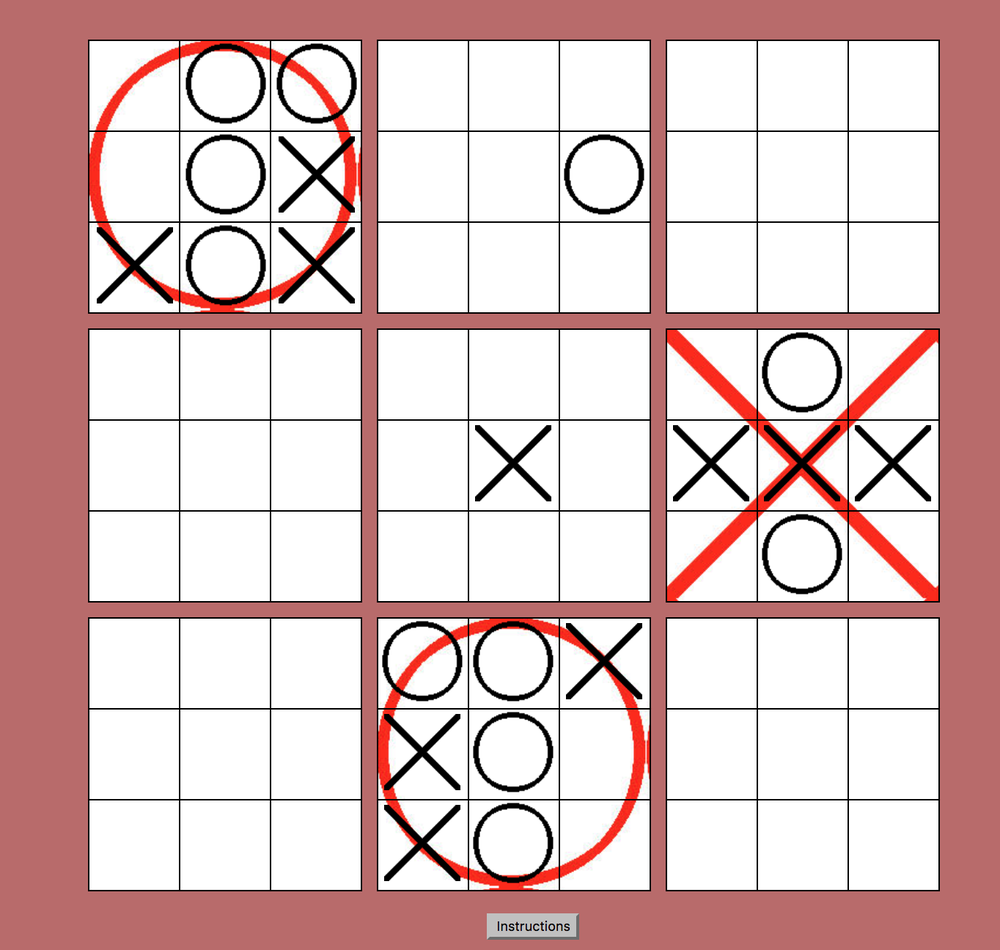
\includegraphics[width=5cm,height=5cm]{tictactoe.png}
\caption{A Ultimate Tic-Tac-Toe game board}
\end{center}
\end{figure}
\\\\
In this paper, we will first analyze 3 different kinds of algorithms and Minimax Algorithm with Alpha-Beta Pruning. We will go ahead to understand why minimax with Alpha-beta pruning is better than others. Although all of the algorithms are known for the Tic-Tac-Toe problem to find the optimal solution, they will be analyzed and compare to find out whether Minimax Algorithm with Alpha-Beta Pruning is the best approach for Tic-Tac-Toe problem. In addition, we will also test a Ultimate Tic-Tac-Toe application to understand how the agent is making decisions all the time, either the agent goes first or second. It is easier to assume if the agent goes second, it will based on how the player moves to calculate the ideal move. However, if the AI goes first, it will be a completely different case, by this we will be able to understand how the algorithm has been coded.
\section{Minimax Algorithm}

According to Borovska and Lazarova, the minimax algorithm is used to determine the optimal move for the agent to play games like zero-sum games since these games can be printed all the possible moves.\cite{Borovska:2007:EPM:1330598.1330615} In addition, they also mentioned that minimax algorithm allows the agent to know that if a move will cost him to lose the game, he will avoid the movie, and if a movie will allow him to win, he will take it and win the game. As we can see, minimax algorithm is almost perfect for a game like Tic-Tac-Toe. However, it relies on having a complete game tree search and lot of time to make one move, said Mathys C. du Plessis.\cite{duPlessis:2009:HNN:1632149.1632158}It will take ages to have a single move for optimality. Despite the fact that how good minimax is, it will not be the best optimization strategy for Tic-Tac-Toe.

\section{Genetic Algorithm}

In the genetic algorithm, our goal is to look for all possible best moves and converge into a winning strategy. In Bhatt et.al , these three authors have achieved to solve an agent that completed a no-loss environment in the Tic-Tac-Toe by using the genetic algorithm. They mentioned that since there is a lot of ways to fill a 3 by 3 grid,39 = 19683, but there are a lot of game states that is infeasible when we tried to rotate the game board for every 90 degrees. By the end, we will end up having 765 unique game states. Since their goal is to develop a no loss strategy, the fitness for the function is defined as the numbers of games lost over the total numbers of games. With the approach from Bhatt et.al, there result in 72657 different strategies in the no-loss strategy. They also mentioned that even though there exist 72657 strategies, many of them will eventually lead to the same game states and do not have a distinct simulation.\cite{Bhatt:2008:SNS:1389095.1389269} Another publication, written by Ferraco et.al from Pennsylvania State University, has developed a 5x5x5 TTT AI implemented by Genetic Algorithm, they also agreed with the strategy that Bhatt and Varshney and Deb, and they further develop to evolve advance TTT for optimizing winning strategy.\cite{ferraco_wang_todd}

\section{Hybrid Neural Network with modified Minimax Algorithm}

For hybrid Neural Network and minimax algorithm, it takes the advantages of minimax algorithm and neural network. Neural network will help to reduce the limited branches which are needed to explore since a neural network can be trained to rank possible moves based on the effectiveness. With the combination, this will allow minimax algorithm to take advantage to make the aggressive move, but also not to make mistakes. According to Mathys C. du Plessis, she created an experiment to test 6 algorithms to have a better win rate versus the others. \cite{Borovska:2007:EPM:1330598.1330615}According to her data, the alpha-beta player, normal neural network player(NN) and hybrid neural network and minimax player(NNM) each played perfectly as first player have a 100\% of the games, while the NNM with selected random branches(MR) and alpha-beta player with selected random branches do lose a quite amount of games. When the agent played as the second player, all of them are losing at least 80\% of the games, but NNM player has won the most game among others, which almost double win rate of the second-best player alpha-beta player. Since the data is given do not provide the information whether NNM is better than normal network(NN), the author ran chi-square test of NNM and NN performed against MR, and it concludes that within 95\% confidence interval that NNM is a better second player than alpha-beta and neural network.\cite{Borovska:2007:EPM:1330598.1330615}

\section{Analyze}

Among these three algorithms, we can expect that minimax is the only that is not include any reduction of game-states. Genetic Approach allows reducing the game states by rotating 90,180, 270 degrees to shorter the equivalence. Hybrid Neural Network with minimax algorithm would do the purpose as the genetic approach. Since using minimax algorithm for Tic-Tac-Toe will represent most of the game states and look for max and min node, it is not a good approach as we cannot shorten the running time for the process. In fact, minimax algorithm with alpha-beta pruning is almost one of the options for Tic-Tac-Toe, but it is not as efficient as the genetic algorithm. To conclude, the genetic approach will be the best approach since it would reduce game states exponentially. In our Ultimate Tic-Tac-Toe, the genetic approach may not be necessary since it does not have a very large game space.
\section{Problem Approach}

As we analyze those three approaches, we understand that any algorithm that enhances the efficiency of minimax algorithm would be a good approach for Ultimate Tic-Tac-Toe. For example, genetic approach and the neural network that we analyze above are also good examples to speed up the process for minimax. However, in our case, it is better to use Alpha-beta pruning for Ultimate Tic-Tac-Toe since it helps to speed the process. The genetic algorithm is not bad at all but in most cases, it would be perfect to use genetic algorithm when we are dealing with a complex game. For Ultimate tic tac toe, it does not have such big search space, the speed up process would not be effective as a complex game. Therefore, we will be using minimax algorithm with alpha-beta pruning for our Ultimate Tic-Tac-Toe. With the use of alpha-beta pruning, we will be able to remove the nodes which do not affect our decision. Let's take about minimax and alpha-beta pruning separately. According to the book written by Stuart Russell, "Artificial Intelligence A Modern Approach", it mentioned minimax algorithm uses a recursive computation of the minimax values of each successor state. It also performs a complete depth-first search exploration of the game tree. Since we know that minimax is a complete depth-first search algorithm, this means that minimax algorithms will find out all the possible moves from the path. With the addition from the Alpha-beta pruning, we will be able to remove the recursive loop for finding unnecessary nodes. Alpha and Beta will be able to store the highest and lowest value along the path. When we understand the node is not fit into the alpha and beta value, we acknowledge that the path is not necessary for our final decision, we can prune it to allow the searching moves fast. In our Ultimate Tic-Tac-Toe case, we have at least 9*$3^9$ combinations of possible moves as original Tic Tac Toe has $3^9$ ways. Since it is a depth-first search game, we can assume that the less deep the depth is, the easier the game will so, which means that we will have less combination that can be gone through.
\section{Design of experiment and Results}

The Ultimate Tic-Tac-Toe that we are going to experiment is created by Mehta-mm. This is an online source code that is written in C++.https://github.com/mehta-mm/Ultimate-Tic-Tac-Toe Although the code is not commented so well that would be easy to understand, I have managed to understand how Mehta has created the algorithm. The algorithm is designed to only allow the bot to start first, and the player will always have to choose O to play the game. Although this code may not be the perfect test subject to examine UTTT, it is the only version that works for me. Under the code, we choose the depth of the depth. The depth was originally set to 6. Since we are testing how would the agent react to decision making, I will be testing at the different level of depth to see what happen. According to the Mehta syntax, the game board is designed from grid 0 to grid 8, which is shown in Figure 2.
\begin{figure}
\begin{center}
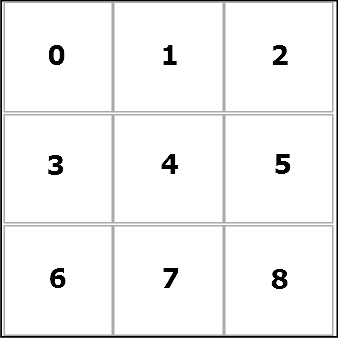
\includegraphics[width=5cm,height=5cm]{0-8_TTT.jpg}
\caption{representation of a Ultimate Tic Tac Toe Game Board}
\end{center}
\end{figure}
\newline

The software has been tested for 8 times so that the player can try to put an O on the fourth grid, which is the middle grid on the 3x3 grid. I have tested for multiple times and confirmed inside the code that the bot's first move will be in the middle of grid four, which is denoted as [4,4]. After the player has placed a move, the bot will be initiated the alpha\_beta function, which triggered the check function that will go through minimax function. The check function will through all the possible path that is available for the next move. When the check function is passed, it will pass through to the alpha\_beta function to update the alpha and beta value. In the end, it will update the value parameter to pass to the final decision.
\newline
\begin{center}
\begin{tabular}{|l|r|}
\hline
Move & Utility Points \\ \hline
0 & 2 \\ \hline
1 & 0\\ \hline
2 & 2 \\ \hline
3 & 0 \\ \hline
4 & 5 \\ \hline
5 & 0 \\ \hline
6 & 2\\ \hline 
7 & 0\\ \hline
8 & 2 \\ \hline
\end{tabular}
\end{center}

This table represents the utility function according to the depth of the game tree = 1, it seems obviously that forth grid is the way to go to make the optimal move.
\newline
\begin{center}
\begin{tabular}{|l|r|}
\hline
Move & Utility Points \\ \hline
0 & 6 \\ \hline
1 & 4\\ \hline
2 & 6 \\ \hline
3 & 4 \\ \hline
4 & 10 \\ \hline
5 & 4 \\ \hline
6 & 6\\ \hline 
7 & 4\\ \hline
8 & 6 \\ \hline
\end{tabular}
\end{center}

This table represents the moves when the depth = 4. As we can see, the agent will choose to pick the 4 grid since it has the highest score.
\newline
\begin{center}
\begin{tabular}{|l|r|}
\hline
Move & Utility Points \\ \hline
0 & 10 \\ \hline
1 & 8\\ \hline
2 & 10 \\ \hline
3 & 8 \\ \hline
4 & 10 \\ \hline
5 & 8 \\ \hline
6 & 10\\ \hline 
7 & 8\\ \hline
8 & 10 \\ \hline
\end{tabular}
\end{center}

For this table, it represents the moves when the depth = 6. However, when we take a closer look, we can see it do not have any unique value to distinguish which grid the bot should take, which takes the bot will eventually have the same equal value for choosing the best moves when the game goes on. To think about it, when the depth of the game tree goes into depth = 4,5,6,7, which means there is a higher chance it is a tie situation when it comes to a tie situation, there mostly do not have many choices to choose, especially we all need to choice losing.
\newline

In fact, based on the software that we tested on, there is some interesting part when Mehta develops the algorithm for it. When the bot is making a move, the result is according to the Utility points. When you get the mark on the mark 4 as Figure 1 on the same board, the score is added 8 points towards the utility. When the bot does not have the mark on grid 4, you will get 4 points deducted. For the bigger grid case, if you won for the middle grid, you will be getting 120 points. And if you won any corner grid, you will get extra 40, such as Grid 0,2,6,8. This is a very interesting case for his algorithm. The above scoring rules allow understanding the bot had prioritized the winning strategy for the game.
\begin{figure}
\begin{center}
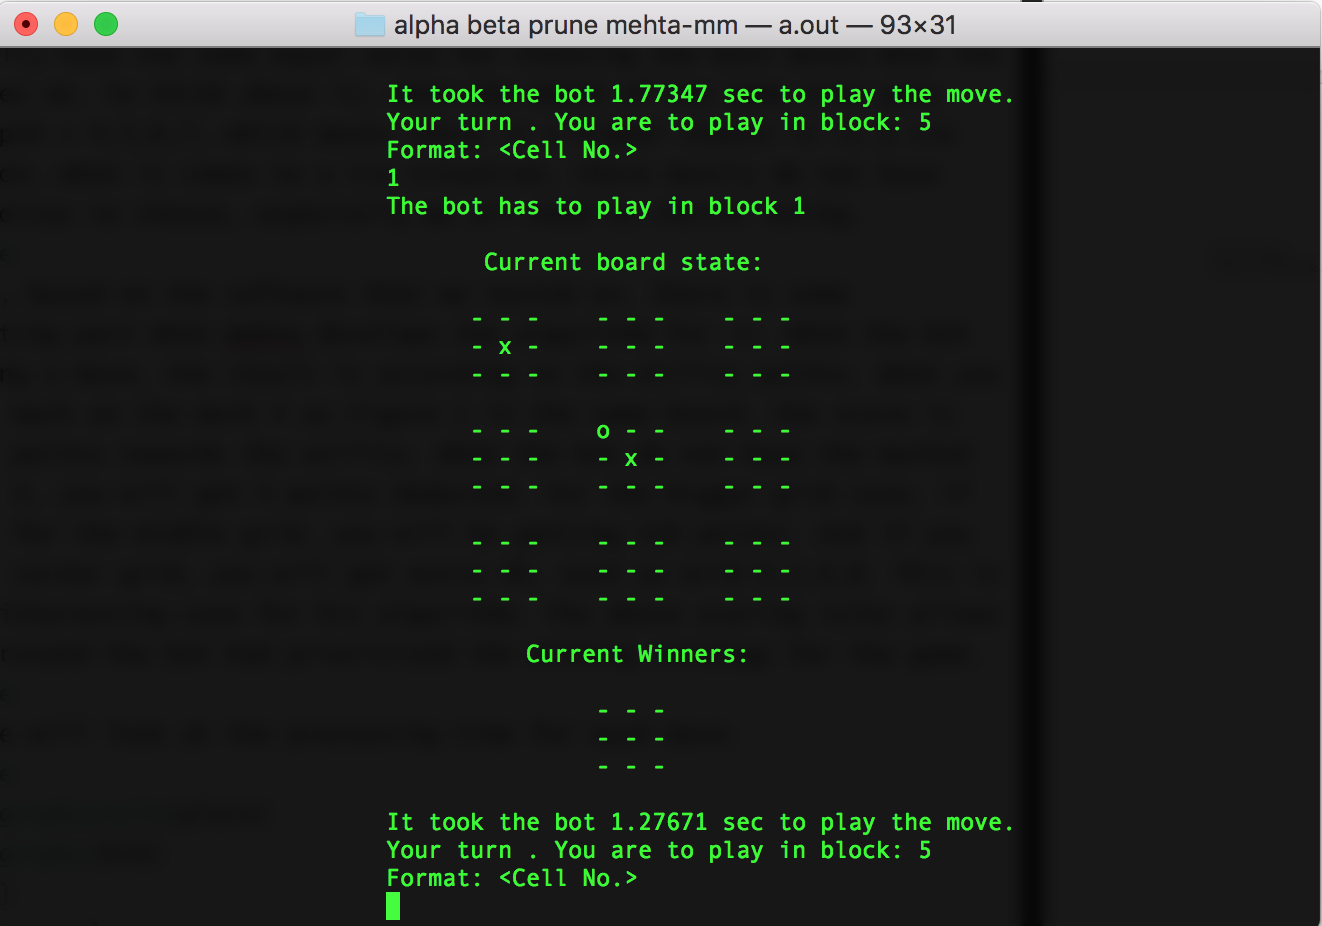
\includegraphics[width=10cm,height=10cm]{ScreenShot.png}
\caption{The interface for the Ultimate Tic Tac Toe gameplay}
\end{center}
\end{figure}
\newline

Next, we will look at the processing time for each move. As we can see from the figure 3, we can that see the agent uses about 1.3 seconds to determine a move, the move is [0,4], which can be explained clearly from above. If the agent would be able to win at the grid 0, there will be extra points for the Utility function, especially the mark 4 on Grid 0 is empty. 8 points will be direct to add to the function. When I tried to test the depth with respect to the time stamp. When the depth of the game tree is deeper, it will use up to 2.5 seconds to make the decisions. In addition, I have used an additional software to help the player side to get the sufficient moves possible in order to perform bot vs bot situation. The game was ended up in a tie situation, and the software that Mehta implemented made a move that uses 2.4975 seconds to make up the decisions.

\section{Analyze}
After running through a lot of testing and examination towards the UTTT implemented by Mehta, we can certainly say that the forth cell which is the middle mark on each grid has the highest chance to win the game when the depth of the game tree is not higher than 4. When the depth of the game tree is higher than 4, the decision making for the agent is extremely hard since there is no any distinct value to compare. It is believed it will be chosen to the first node of the highest score. Let's take the example from Table2, there are 5 10-point cells, and 4 8-point cells. In this case, the agent will definitely take 10-points. However, there is the question. There are five options that the agent can choose. Under my observation, if the fourth cell is still empty, the choice will definitely go to the fourth cell. If this is not the case, it is believed it will choose the first node of 10-points cell, which is cell 0. The reason behind this because the software is implemented in C++, C++ syntax when the data points are the same, it will directly go to first one according to the memory address. Once they have decided the right grid, it will go to the player's move. After the player takes the move, the utility points for the depth will change again, so that at each turn, there would be a different scoreboard to decide which is the right move. Nonetheless, the strategy for the agent winning the game is unchanged. The bot will try to capture the middle cell at every grid and conquer the corner grid, such as top left and right and bottom left and right. 
\newline

In addition, when we look at those three tables, we can observe that the shallower the depth of the game tree is, the easier the decision will be. In table 1, it is clear that cell 4 is the optimal move to make when depth = 1. However, let's look at table 3, where the depth of the game tree will increase to 6. There is only 2 distinct value to choose, 10 and 8 points. We can imagine when the depth of the game tree goes deeper such as 8 or 10, it may result in no distinct values. The reason why the game tree goes in that deep is that there are no many choices to make and the game has half-way done. In that case, the agent only cares about whether not to make wrong decisions to allow the player to win the game. For example, trying to make the game to a tie situation. Professor Hochmuth also mentioned that the best strategy to win a game is to avoid losing.\cite{hochmuth_2003} However, the only disadvantage of this implementation is that it cannot avoid double win situation. For example, when a move allows the agent to win a grid, but also allow the player to win a grid right after the agent makes the optimal move. Although it is optimal for the agent, it is also one of the bad moves that the agent did not realize. It is extremely difficult to create an unbeatable to take care of prediction. To be honest, the bad moves may not be so important for the agent because the unbeatable agent will almost never make any mistakes, while players as human will always make careless mistakes, even we tried our best to avoid it. When we made a mistake, we will probably give a lead to the bot. However, if we made two mistakes, we are screwed, ready to lose a game.
\section{Conclusion}
In this paper, we analyze many different algorithms that will help to speed up the process of minimax algorithm. We acknowledge that genetic algorithm will be the fastest way to reduce the time for each decision making. However, it will not be optimal in Ultimate Tic-Tac-Toe. Therefore, we will use minimax algorithm with alpha-beta pruning to reduce the timestamps effectively. We will also observe the test results from the online source code to compare the results with different depth. By observing the different depth of the game tree, we will be able to understand how the agent makes the right decisions, and how the depth will affect the cost of time. Lastly, we also pointed some disadvantages that the agent will potentially make.
\newpage
\bibliographystyle{plain}
\bibliography{bib}
\cite{*}
\end{document}
